\documentclass[a4paper,12pt]{article}

\usepackage{cmap}                      % Поддержка поиска русских слов в PDF (pdflatex)
\usepackage[utf8]{inputenc}            % Выбор языка и кодировки
\usepackage[english, russian]{babel}

\usepackage[usenames]{color}

\usepackage[matrix,arrow,curve]{xy}
\usepackage[mathcal]{eucal}
\usepackage{amsfonts,amsmath,amsthm,graphicx,amssymb}
\usepackage[noend]{algorithmic}
\usepackage[caption]{algorithm}

\usepackage[left=3cm,right=2cm,top=2cm,bottom=2cm]{geometry} % поля страницы

\usepackage[pdftex]{hyperref}

\graphicspath{{../../images/}} 			% Пути к изображениям

\usepackage[
	language=auto,
	autolang=other,
	backend=biber,
	style=authortitle,
	sorting=ydnt,
	maxbibnames=5
]{biblatex}
\addbibresource{semnet.bib}

\begin{document}

\newtheorem{Th}{Теорема}
\newtheorem{Def}{Определение}
\newtheorem{Pred}{Утверждение}
\floatname{algorithm}{Алгоритм}

\author{А.И. Панов}
\title{Структурная модель картины мира когнитивного агента}

\maketitle{}

% оформление аннотации
\begin{abstract}
Основная цель настоящей работы описать математическую модель картины мира когнитивного агента на структурном уровне. 
\end{abstract}

\section{Каузальная матрица}

Рассмотрим следующую структуру - кортеж $\bar z=(e_1, e_2,\dots,e_h)$, состоящий из битовых векторов $e_i$ одинаковой длины $q$. Введем типизацию элементов кортежа $\bar z$: первые $t_c$ столбцов будут иметь тип $\lambda_c$, оставшиеся $t_e=h-t_c$ столбцов - тип $\lambda_e$. Иными словами, задана функция $\Lambda$, которая множеству индексов элементов кортежа $I(\bar z)$ ставит в соответствие тип элемента $\Lambda: I(\bar z)\rightarrow \{\lambda_x,\lambda_e\}$. Так как все элементы кортежа $\bar z$ типа $\lambda_c$ идут первыми и подряд, то можно так же сказать, что кортежу $\bar z$ соответствует порог $t_c(\bar z)$: $\forall i\leq t_c$ элементы $e_i$ имеют тип $\lambda_c$, а $\forall t_c<i\leq h$ - тип $\lambda_e$. Особым случаем является случай $t_c=h$, означающий, что элементов типа $\lambda_e$ в кортеже $\bar z$ нет.

\begin{Def}
Каузальной матрицей $z$ будем называть пару $\langle\bar z, \bar n\rangle$, где $\bar n=(n_1,n_2,\dots,n_q)$ - вектор той же длины $q$, что и элементы $e_i$ кортежа $\bar z$. Элементы $e_i$ кортежа $\bar z$ будем называть событиями, а элементы $n_j$ вектора $\bar n$ - именами признаков или просто признаками. 
\end{Def}

Таким образом, каузальная матрица $z$ является битовой матрицей размерности $h\times q$, в которой выделяются два типа столбцов: столбцы типа $\lambda_c$ (будем называть их столбцами-условиями) и столбцы типа $\lambda_e$ (будем называть их столбцами-эффектами). Схематическое изображение данной конструкции представлено на рис.~\ref{fig:causmatr}.

С точки зрения распознавания образов структура каузальной матрицы $z=\langle\bar z, \bar n \rangle$, хранящая образ некоторой сущности, интерпретируется следующим образом. Каждый столбец $e_i$  (битовый вектор кортежа $\bar z$) задает множество признаков $N_i$, состоящее из элементов вектора $\bar n$), которые должны присутствовать в момент времени $i$ для успешного распознавания представляемой сущности: $N_i=\{n_j|n_j\in \bar n \land e_i(j)=1\}$. В том случае, когда в каузальной матрице нет столбцов условий, представляемая сущность является статическим объектом, в противном случае - динамическим процессом или действием. Соответственно, столбцы-условия задают образ условий данного действия, а столбцы-эффекты - образ эффектов.

\begin{figure}[H]
	\centering
	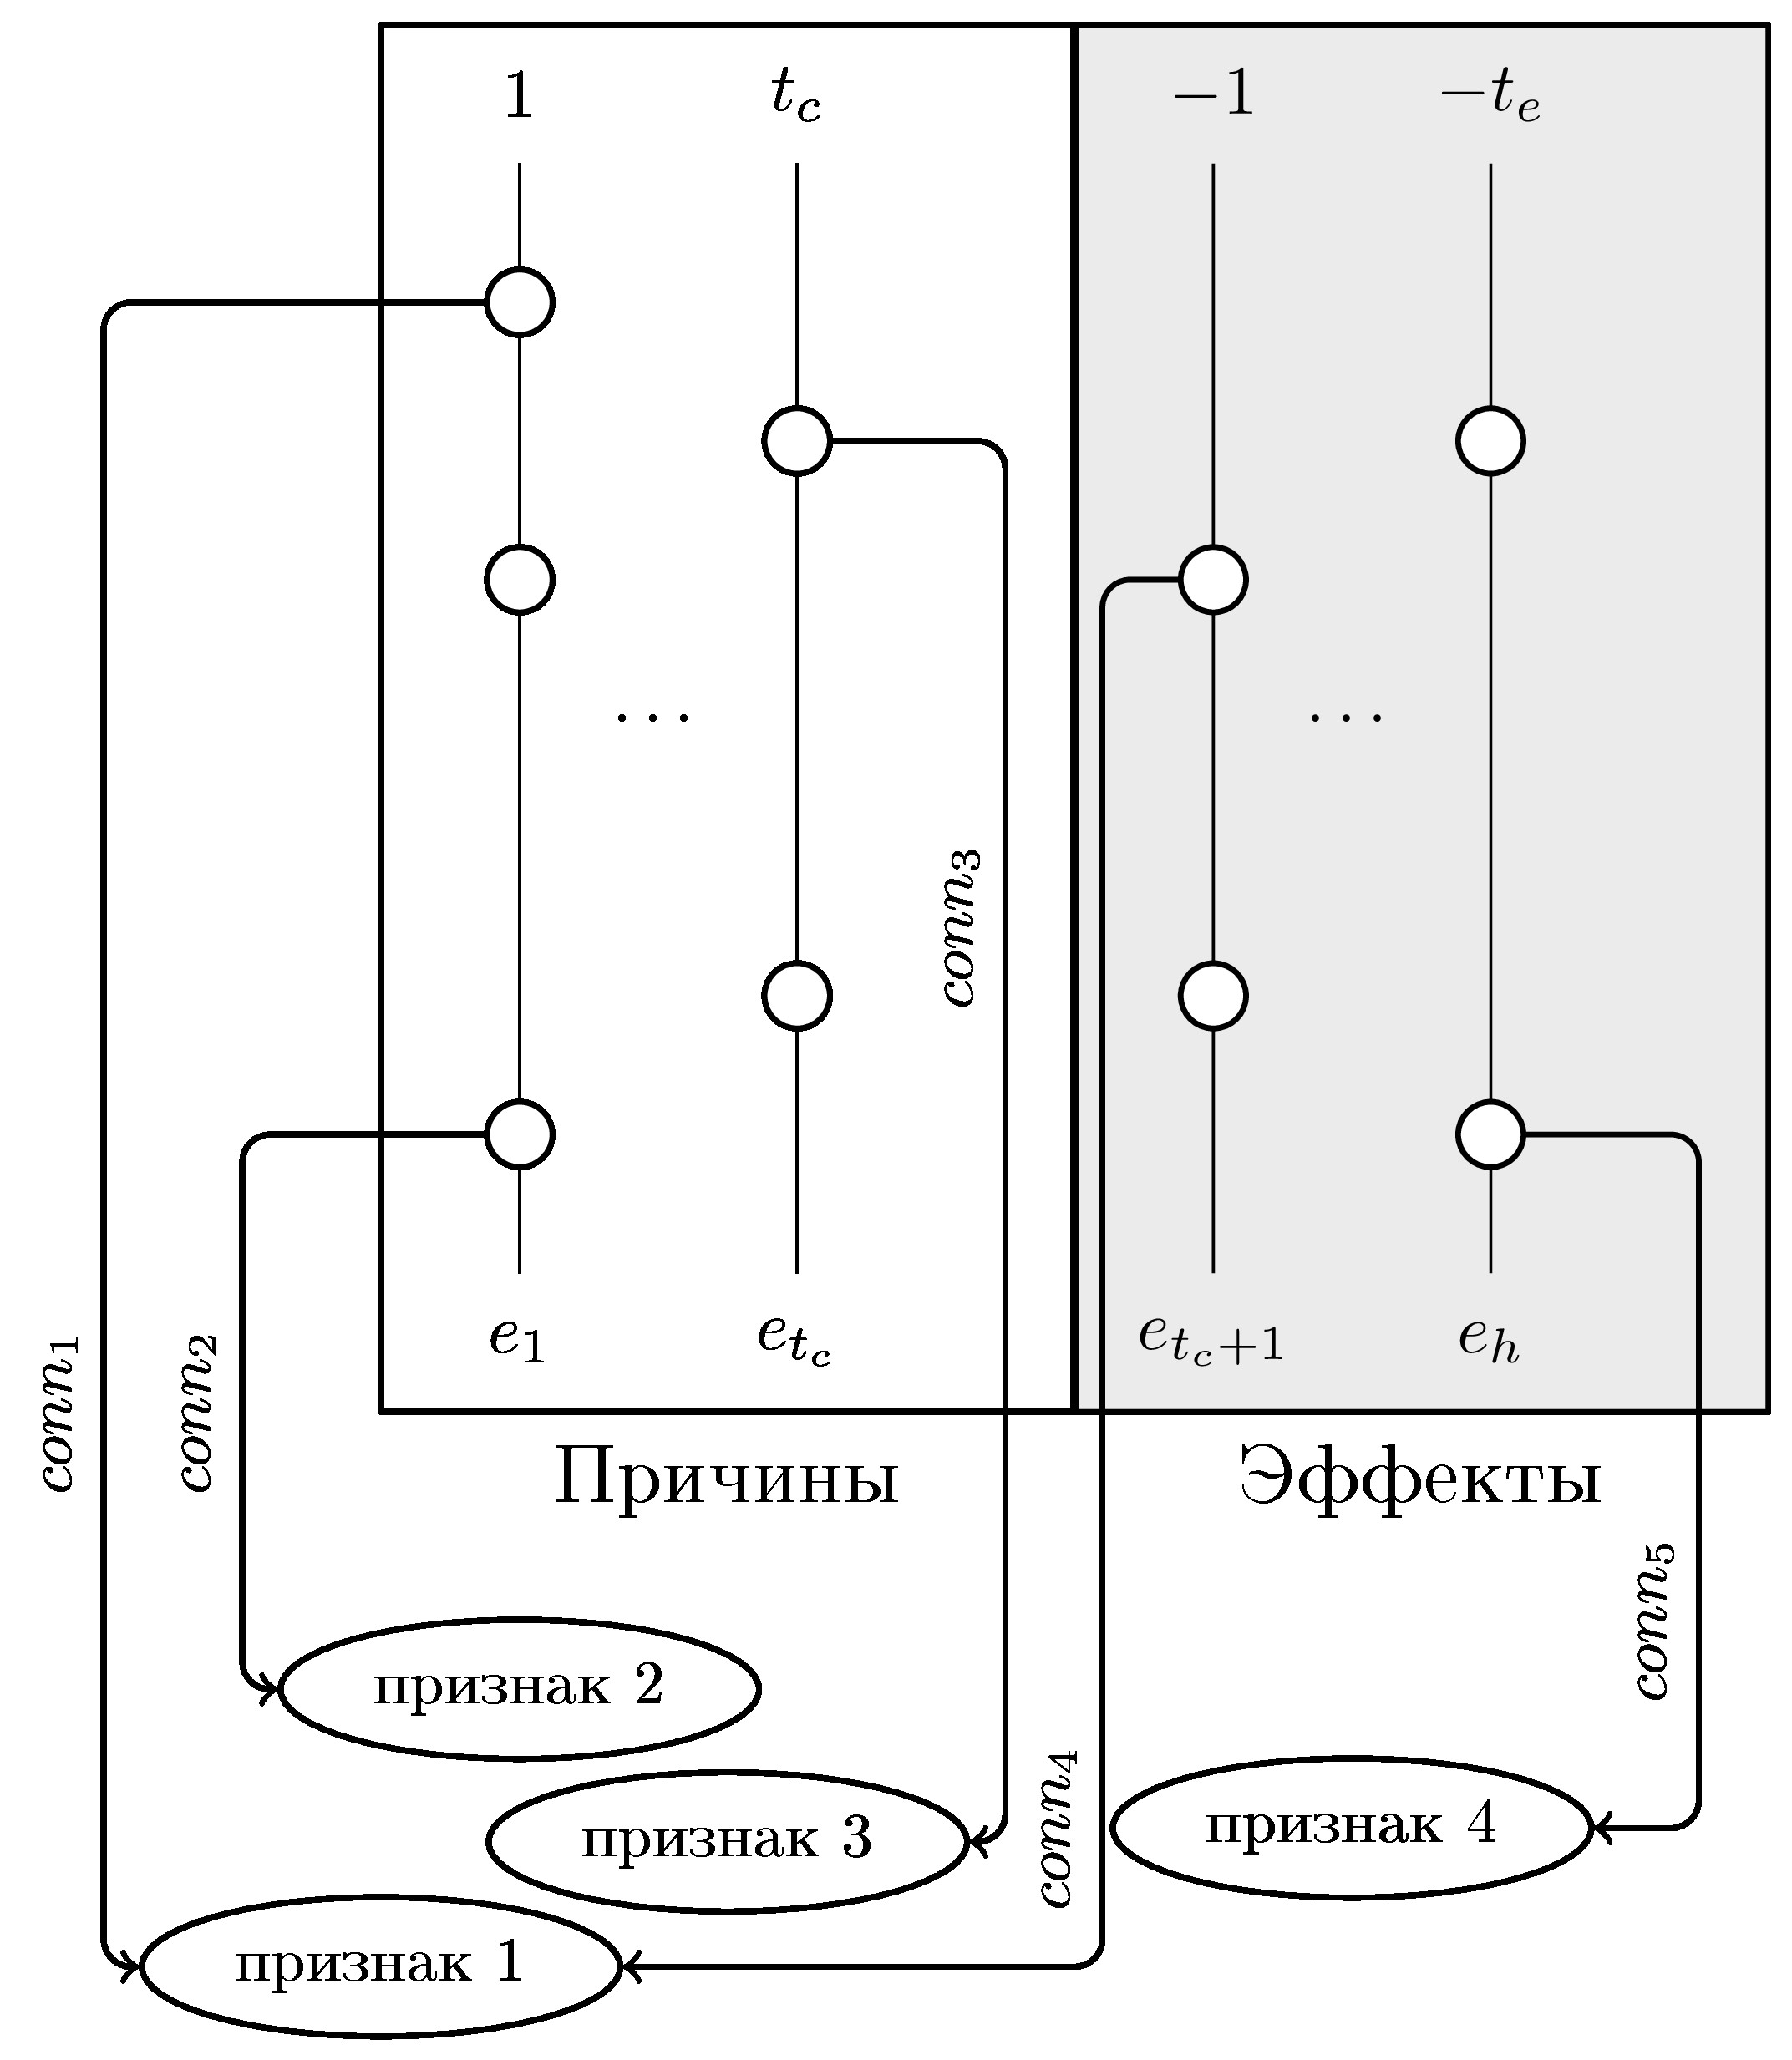
\includegraphics[width=0.5\textwidth]{causnet/caus_matr2_ru.jpg}
	\label{fig:causmatr}
	\caption{Схема каузальной матрицы $z$}
\end{figure}

В качестве примера приведем матрицу $z=\langle \bar z, \bar n\rangle$, где кортеж $\bar z$ записывается в виде диагональной матрицы размера $4\times 4$, а вектор $\bar n$ равен вектору $(\text{левый глаз}, \text{правый глаз}, \text{нос}, \text{рот})$.
\section{Каузальная сеть}
Про распространение активности

\section{Семиотическая сеть}
Про неподвижную точку оператора

\begin{Th}[необходимое условие сходимости]
	Процесс 
\end{Th}

\section{Когнитивные функции}


\nocite{*}
\printbibliography[keyword={strl}, resetnumbers=true]
\end{document} 